  ПО для онлайн монитора светимости работает на выделенном компьютере. Считывающие ПО запущенное на данном компьютере непрерывно считывает данные из модуля LOM и позволяет получать значения светимости в локальной сети, а также отправляет полученные значения в системы медленного контроля (Рис. 8). Поскольку поток данных с монитора светимости составляет приблизительно 35 Кб/с, то не накладывается строгих ограничений на производительность считывающего ПО и ПО мониторинга. В связи с этим Python был выбран в качестве основного языка для написания большей части програмного обеспечения.\par
  Считывающее ПО представляет собой многопоточный TCP-сервер и работает как прокси для модуля монитора светимости. Поскольку программа монитора светимости является однопоточной, одной из важных функций считывающего ПО является обеспечение обработка поступающих параллельно входящих запросов и предотвращение возможных сбоев прошивки, вызванных несколькими одновременными запросами к монитору светимости. Он также кэширует данные, которые могут запрашиваться клиентскими приложениями, тем самым сокращая количество операций считывания и повышая общую производительность.\par
  Для дальнейшей передачи данных сервер LOM использует библиотеку pythonIOC, встроенный сервер доступа к каналам (Channel Access, CA) EPICS, что делает всю информацию о светимости доступной в системе медленного контроля Belle II. Помимо значений мгновенной светимости, он также производит расчет интегральных и максимальных светимостей, значений пьедесталов, обеспечивает сохранность данных о которых будет описано подробнее в следующей главе.
\begin{figure}[htp]
  \centering
  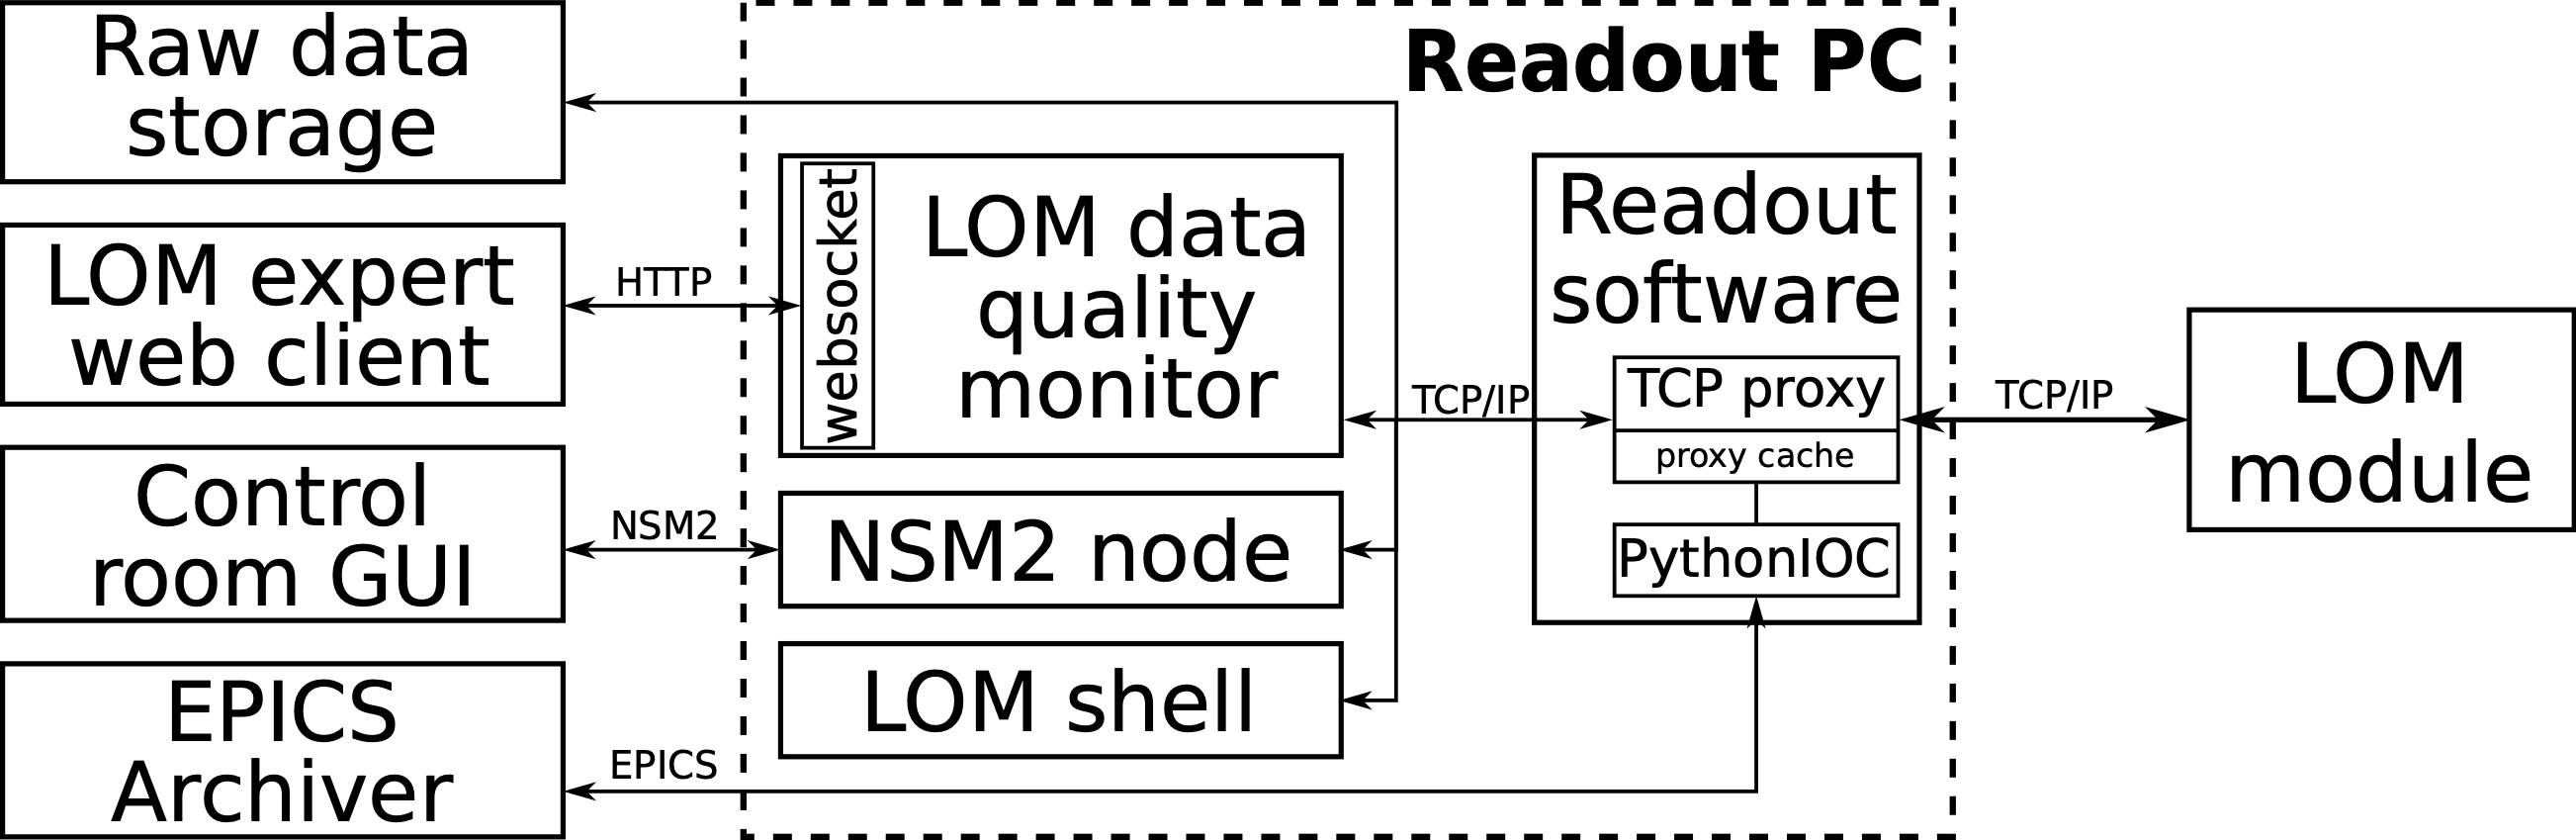
\includegraphics[width=\textwidth]{LOM_software.pdf}
  \caption{Схема архитектуры ПО}
  \label{fig:galaxy}
\end{figure}
